% Chapter 6: Analysis
\section{性能对比分析}

\subsection{实验结果汇总}

表\ref{tab:summary}汇总了三类数据集上的主要实验结果。

\begin{table}[htbp]
    \centering
    \caption{实验结果汇总}
    \label{tab:summary}
    \begin{tabular}{llcccc}
        \toprule
        \textbf{数据集} & \textbf{索引} & \textbf{树高} & \textbf{构建距离} & \textbf{最佳范围剪枝} & \textbf{最佳kNN剪枝} \\
        \midrule
        \multirow{2}{*}{蛋白质(1,469)} & GH-Tree & 8 & 28,461 & 57.7\% & 60.6\% \\
                                        & VP-Tree & 6 & 11,682 & 71.7\% & 79.3\% \\
        \midrule
        \multirow{2}{*}{低维2D(10,000)} & GH-Tree & 15 & 290,202 & -6.8\% & 99.0\% \\
                                         & VP-Tree & 8 & 92,248 & 0.0\% & 99.2\% \\
        \midrule
        \multirow{2}{*}{高维20D(5,000)} & GH-Tree & 15 & 128,412 & -6.6\% & -6.6\% \\
                                         & VP-Tree & 7 & 41,103 & 0.0\% & 0.0\% \\
        \bottomrule
    \end{tabular}
\end{table}

\subsection{不同数据集上的性能差异分析}

\subsubsection{蛋白质序列数据分析}

蛋白质序列数据集上,VP树表现明显优于GH树:

\begin{itemize}
    \item \textbf{构建效率}:VP树构建距离计算仅为GH树的41\%(11,682 vs 28,461)
    \item \textbf{树结构}:VP树更平衡(高度6 vs 8)
    \item \textbf{范围查询}:VP树剪枝率更高(71.7\% vs 57.7\%)
    \item \textbf{kNN查询}:VP树优势更明显(79.3\% vs 60.6\%)
\end{itemize}

\textbf{原因分析}:
\begin{enumerate}
    \item 蛋白质序列的Alignment距离具有较好的区分度
    \item VP树的距离范围信息能更精确地描述子树中数据的分布
    \item GH树需要两个pivot,构建开销更大
\end{enumerate}

\subsubsection{低维向量数据分析}

低维向量数据集的特点:

\begin{itemize}
    \item \textbf{范围查询}:两种树剪枝效果都不佳,GH树甚至出现负剪枝(-6.8\%)
    \item \textbf{kNN查询}:两种树都表现优异,剪枝率超过98\%
    \item \textbf{树高差异}:GH树(15层)远高于VP树(8层)
\end{itemize}

\textbf{原因分析}:
\begin{enumerate}
    \item 范围查询的半径相对数据分布较大,导致大部分子树都需要访问
    \item GH树的负剪枝来自于每个内部节点需要计算到2个pivot的距离
    \item kNN查询随着搜索进行,动态半径不断缩小,剪枝效果逐渐显现
    \item 聚类分布的数据可能导致GH树超平面划分不均
\end{enumerate}

\subsubsection{高维向量数据分析}

高维向量数据集展现了严重的"维度灾难"现象:

\begin{itemize}
    \item \textbf{范围查询}:两种树几乎无法剪枝
    \item \textbf{kNN查询}:同样无法有效剪枝
    \item \textbf{构建开销}:GH树距离计算仍是VP树的3倍
\end{itemize}

\textbf{原因分析}:
\begin{enumerate}
    \item 高维空间中,数据点之间的距离趋于相近(距离集中现象)
    \item 三角不等式提供的剪枝边界变得松散
    \item 球形区域在高维空间中体积占比急剧上升
\end{enumerate}

\subsection{性能差异的原因分析}

\subsubsection{数据划分方式的影响}

图\ref{fig:partition-comparison}展示了两种划分方式的差异。

\begin{figure}[htbp]
    \centering
    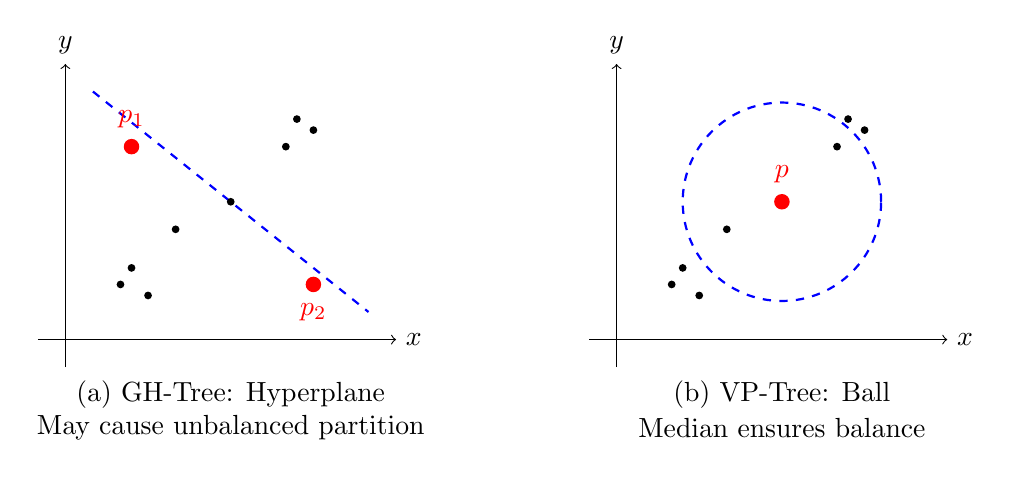
\begin{tikzpicture}[scale=0.7]
        % GH Tree partition
        \begin{scope}[xshift=0cm]
            \draw[->] (-0.5,0) -- (6,0) node[right] {$x$};
            \draw[->] (0,-0.5) -- (0,5) node[above] {$y$};
            
            % Hyperplane (diagonal)
            \draw[thick,blue,dashed] (0.5,4.5) -- (5.5,0.5);
            
            % Data points (clustered)
            \foreach \x/\y in {1/1, 1.2/1.3, 1.5/0.8, 4/3.5, 4.2/4, 4.5/3.8, 2/2, 3/2.5} {
                \fill[black] (\x,\y) circle (2pt);
            }
            
            \fill[red] (1.2,3.5) circle (4pt);
            \fill[red] (4.5,1) circle (4pt);
            \node[red] at (1.2,4) {$p_1$};
            \node[red] at (4.5,0.5) {$p_2$};
            
            \node at (3,-1) {(a) GH-Tree: Hyperplane};
            \node at (3,-1.6) {May cause unbalanced partition};
        \end{scope}
        
        % VP Tree partition
        \begin{scope}[xshift=10cm]
            \draw[->] (-0.5,0) -- (6,0) node[right] {$x$};
            \draw[->] (0,-0.5) -- (0,5) node[above] {$y$};
            
            % Ball boundary
            \draw[thick,blue,dashed] (3,2.5) circle (1.8);
            
            % Data points (clustered)
            \foreach \x/\y in {1/1, 1.2/1.3, 1.5/0.8, 4/3.5, 4.2/4, 4.5/3.8, 2/2, 3/2.5} {
                \fill[black] (\x,\y) circle (2pt);
            }
            
            \fill[red] (3,2.5) circle (4pt);
            \node[red] at (3,3) {$p$};
            
            \node at (3,-1) {(b) VP-Tree: Ball};
            \node at (3,-1.6) {Median ensures balance};
        \end{scope}
    \end{tikzpicture}
    \caption{两种划分方式对比}
    \label{fig:partition-comparison}
\end{figure}

\begin{itemize}
    \item \textbf{GH树}:超平面位置取决于两个pivot的选择,可能导致不平衡划分
    \item \textbf{VP树}:使用中位数划分,保证两个子树大小相等
\end{itemize}

\subsubsection{支撑点使用效率的影响}

\begin{table}[htbp]
    \centering
    \caption{支撑点使用效率对比}
    \label{tab:pivot-efficiency}
    \begin{tabular}{lcc}
        \toprule
        \textbf{指标} & \textbf{GH树} & \textbf{VP树} \\
        \midrule
        每节点pivot数 & 2 & 1 \\
        构建时距离计算/节点 & $\sim 2n$ & $\sim n$ \\
        查询时距离计算/节点 & 2 & 1 \\
        存储的剪枝信息 & 无 & 距离范围$[L,U]$ \\
        \bottomrule
    \end{tabular}
\end{table}

VP树的优势:
\begin{enumerate}
    \item 每个节点只需一个pivot,减少构建和查询的距离计算
    \item 存储距离范围,提供更精确的剪枝信息
    \item 一次距离计算可以同时用于两个子树的剪枝判断
\end{enumerate}

\subsubsection{数据分布特征的影响}

\begin{itemize}
    \item \textbf{聚类数据}:GH树的超平面可能穿过聚类,导致相似数据分离;VP树的球形划分更能保持聚类完整
    \item \textbf{均匀数据}:两种树表现相近
    \item \textbf{高维数据}:两种树都受维度灾难影响
\end{itemize}

\subsubsection{维度灾难的影响}

维度灾难(Curse of Dimensionality)是高维数据处理的核心挑战:

\begin{enumerate}
    \item \textbf{距离集中}:高维空间中,点与点之间的距离趋于相近
    \item \textbf{剪枝失效}:三角不等式提供的边界变得松散
    \item \textbf{体积增长}:高维球的体积相对整个空间的占比极大
\end{enumerate}

图\ref{fig:dimension-curse}展示了维度对剪枝效果的影响。

\begin{figure}[htbp]
    \centering
    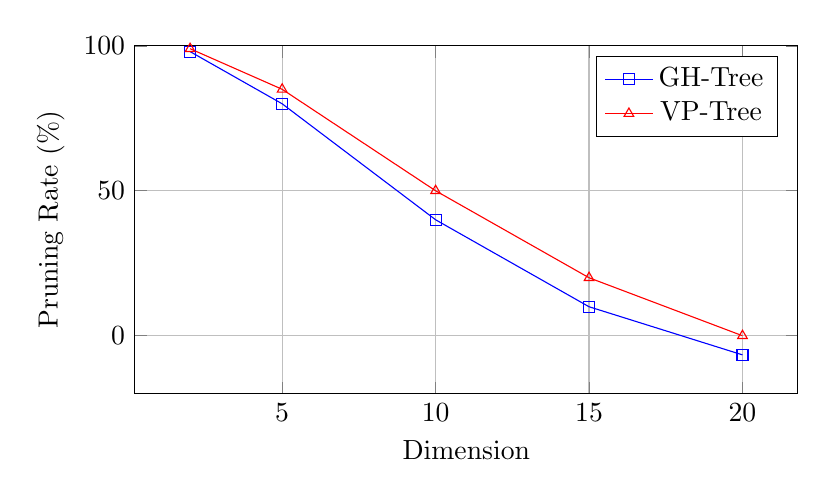
\begin{tikzpicture}
        \begin{axis}[
            width=10cm,
            height=6cm,
            xlabel={Dimension},
            ylabel={Pruning Rate (\%)},
            legend pos=north east,
            grid=major,
            ymin=-20,
            ymax=100
        ]
        \addplot[color=blue,mark=square] coordinates {
            (2, 98) (5, 80) (10, 40) (15, 10) (20, -6.6)
        };
        \addplot[color=red,mark=triangle] coordinates {
            (2, 99) (5, 85) (10, 50) (15, 20) (20, 0)
        };
        \legend{GH-Tree, VP-Tree}
        \end{axis}
    \end{tikzpicture}
    \caption{维度对剪枝效果的影响(示意图)}
    \label{fig:dimension-curse}
\end{figure}

\subsection{GHT与VPT的优缺点总结}

\subsubsection{GHT的优势与局限}

\textbf{优势}:
\begin{itemize}
    \item 超平面划分在某些低维数据上可能更有效
    \item 概念简单直观
    \item 在数据分布均匀时划分效果好
\end{itemize}

\textbf{局限}:
\begin{itemize}
    \item 需要2个pivot,构建开销大
    \item 每次查询需计算到2个pivot的距离
    \item 划分可能不平衡
    \item 无法利用距离范围信息进行精确剪枝
\end{itemize}

\subsubsection{VPT的优势与局限}

\textbf{优势}:
\begin{itemize}
    \item 只需1个pivot,构建更高效
    \item 中位数划分保证树的平衡性
    \item 距离范围信息提供精确剪枝
    \item 在多种数据集上表现稳定
\end{itemize}

\textbf{局限}:
\begin{itemize}
    \item 球形划分在某些数据分布下效率不高
    \item 高维数据上同样受维度灾难影响
    \item 需要额外存储距离范围信息
\end{itemize}

\subsubsection{适用场景分析}

\begin{table}[htbp]
    \centering
    \caption{GH树和VP树的适用场景}
    \label{tab:use-cases}
    \begin{tabular}{lcc}
        \toprule
        \textbf{场景} & \textbf{推荐索引} & \textbf{原因} \\
        \midrule
        低维均匀数据 & 均可 & 两者表现相近 \\
        低维聚类数据 & VP-Tree & 保持聚类完整性 \\
        高维数据 & 均不推荐 & 维度灾难 \\
        序列数据 & VP-Tree & 更好的剪枝效果 \\
        构建时间敏感 & VP-Tree & 构建更快 \\
        内存受限 & GH-Tree & 无需存储距离范围 \\
        \bottomrule
    \end{tabular}
\end{table}

\subsection{改进方向讨论}

\subsubsection{Pivot选择策略优化}

当前的FFT策略虽然比随机选择更好,但仍有改进空间:

\begin{enumerate}
    \item \textbf{基于样本的选择}:从数据采样中选择方差最大的pivot组合
    \item \textbf{增量式选择}:根据已有pivot的效果动态调整
    \item \textbf{自适应策略}:根据数据分布特征选择不同策略
\end{enumerate}

\subsubsection{树结构平衡性优化}

\begin{enumerate}
    \item \textbf{GH树}:引入平衡因子,在划分不均时调整pivot选择
    \item \textbf{动态重构}:定期检测并重新平衡不平衡的子树
    \item \textbf{多路划分}:扩展为k路划分,增加灵活性
\end{enumerate}

\subsubsection{多路划分扩展}

将二叉划分扩展为多路划分可能提高效率:

\begin{itemize}
    \item \textbf{GHT扩展}:使用多个pivot定义多个超平面
    \item \textbf{VPT扩展}:使用多个同心球划分(MVP树)
\end{itemize}

\subsubsection{动态索引维护}

当前实现只支持批量构建。未来可以扩展:

\begin{enumerate}
    \item \textbf{增量插入}:支持单个数据的插入
    \item \textbf{删除操作}:支持数据删除和懒惰删除
    \item \textbf{自适应重构}:当索引效率下降时自动重构
\end{enumerate}

\subsubsection{高维数据优化}

针对高维数据的特殊优化:

\begin{enumerate}
    \item \textbf{降维预处理}:使用PCA等方法降维后再建索引
    \item \textbf{近似查询}:牺牲精确性换取效率
    \item \textbf{混合索引}:结合哈希等方法
\end{enumerate}

